% Online Resource 2: sensitivity analysis of the architecture ranking.
% Tables are \input from ../../sensitivity/, written by code/sensitivity.py, so no number is
% retyped. Build after the main paper, so that ../main.aux resolves the \ref{M-...} labels.
\documentclass[11pt]{article}
\usepackage[margin=2.3cm]{geometry}
\usepackage{booktabs}
\usepackage{array}
\usepackage{graphicx}
\usepackage{amsmath,amssymb}
\usepackage{xr}
\usepackage[round]{natbib}
\usepackage{url}
\externaldocument[M-]{../main}
\graphicspath{{../../sensitivity/}}
\renewcommand{\thetable}{S\arabic{table}}
\renewcommand{\thefigure}{S\arabic{figure}}
\renewcommand{\thesection}{S\arabic{section}}
\newcolumntype{L}[1]{>{\raggedright\arraybackslash}p{#1}}
% LaTeX's \input is not expandable inside a tabular; the primitive is.
\makeatletter\newcommand{\tabinput}[1]{\@@input #1 }\makeatother

\title{Online Resource 2\\[0.4em]
\large Carbon Footprint and Carbon-Aware Selection of Document-Oriented, Relational, and Hybrid Object-Relational Storage for Image-Based Time-Series Workloads in Green IoT\\[0.4em]
\normalsize Sensitivity analysis of the architecture ranking}
\author{[Authors hidden for double-blind review]}
\date{}

\begin{document}
\maketitle

\noindent Section and table numbers marked ``main text'' refer to the manuscript; those prefixed with S refer to this document. Every value here is computed from the measurement files released with the artifact by \texttt{code/sensitivity.py}, which writes its results to \texttt{sensitivity/}; no benchmark was re-run.

\section{What is varied, and how}\label{sec:method}
Each factor on which the ranking could plausibly depend is varied on its own, and for each the question is the same: does the lowest-carbon architecture change, and at which payload? The analysis uses the measured cells of all six data sets: the collage sweep on the larger host (i9, 360p to 6K) and on the smaller host (i7, 360p to 6K), the real frames of each of the three cameras on the smaller host (360p to 1080p for the networked and USB cameras, 360p to 720p for the built-in one), and the three cameras interleaved at 1080p. Carbon values are the amortised per-run figures of the main text (Section~\ref{M-subsec:carbon_method}), and cells recorded as skipped are excluded before anything else, since a failed cell still leaves a partial tracker in the emissions log. Table~\ref{tab:summary} summarises the outcome; it is also Table~\ref{M-tab:robustness} of the main text.

\begin{table}[htbp]
\centering
\caption{Summary: does the choice of architecture change?}\label{tab:summary}
\small
\begin{tabular}{@{}L{0.19\textwidth}L{0.32\textwidth}L{0.4\textwidth}@{}}
\toprule
Factor & Range tested & Does the choice change? \\
\midrule
Operation mix & 0 to 10 bulk retrievals and 0 to 2{,}000 latest-frame reads per 2{,}000 inserts & Collage, either host: no. Real frames: only at the networked camera's 1080p payload, where inline PostgreSQL wins up to 0.5 bulk retrievals and 100 latest-frame reads, and MongoDB beyond (Section~\ref{sec:mix}) \\
Run-to-run variability & Each operation perturbed by its own run-to-run spread & No winner overturned on the larger host; nine cells at a crossover on the smaller host become ties (Section~\ref{sec:variability}) \\
Embodied carbon of retained frames & 0.02 (HDD) and 0.16 (SSD) kg CO$_2$eq per GB, 30 to 365 days at 5 frames per second & Only where the operational winner keeps more bytes on disk than a close rival, most notably at the deployment payload (Section~\ref{sec:embodied}) \\
Grid intensity & 41 to 713 g CO$_2$eq/kWh, seven national grids & No: every architecture scales by the same factor (Section~\ref{sec:grid}) \\
Facility overhead (PUE) & 1.0 to 2.0 & No, for the same reason \\
Frame rate and camera count & Any & No: both scale every architecture linearly (Section~\ref{sec:scale}) \\
Host and corpus & Two hosts; collage and three real cameras & The ordering holds; the crossover moves (Section~\ref{sec:host}) \\
\bottomrule
\end{tabular}
\end{table}

\section{Operation mix}\label{sec:mix}
The main text reports two operation profiles: ingestion only, and an equal-weight profile counting one insertion run of 2{,}000 frames, one bulk retrieval of those frames, and one latest-frame read. Real workloads lie between and beyond these. The carbon of storing 2{,}000 frames is therefore written as $I + bR + pP$, where $I$, $R$ and $P$ are the measured insertion, bulk-retrieval and latest-frame-read carbon of one run, $b$ is the number of bulk retrievals and $p$ the number of latest-frame reads per 2{,}000 inserts. We take $b$ from 0 to 10 and $p$ from 0 to 2{,}000, the upper value being one dashboard read for every stored frame.

On the collage the answer never changes. On both hosts and at every payload, the same architecture is greenest under every mix (Table~\ref{tab:mix}, Figure~\ref{fig:mix}): the crossover is set by insertion, and reads only scale the margin. On real frames the mix matters at one payload. At the networked camera's 1080p, inline PostgreSQL is greenest for ingestion-heavy workloads, up to half a bulk retrieval and 100 latest-frame reads per 2{,}000 inserts, and MongoDB for anything more read-heavy. At 720p, one latest-frame read per stored frame is enough for PostgreSQL's cheaper point read to win, an edge case of little practical weight. The other two cameras and the interleaved run select MongoDB under every mix.

\begin{table}[htbp]
\centering
\caption{Greenest architecture by payload under four operation mixes. Mixes are given per 2{,}000 inserts.}\label{tab:mix}
\footnotesize
\begin{tabular}{@{}L{0.14\textwidth}L{0.19\textwidth}L{0.19\textwidth}L{0.19\textwidth}L{0.19\textwidth}@{}}
\toprule
Data set & Ingestion only & Equal weight & 10 bulk retrievals & 2{,}000 latest-frame reads \\
\midrule
\tabinput{../../sensitivity/tab_mix.tex}
\bottomrule
\end{tabular}
\end{table}

\begin{figure}[htbp]
\centering
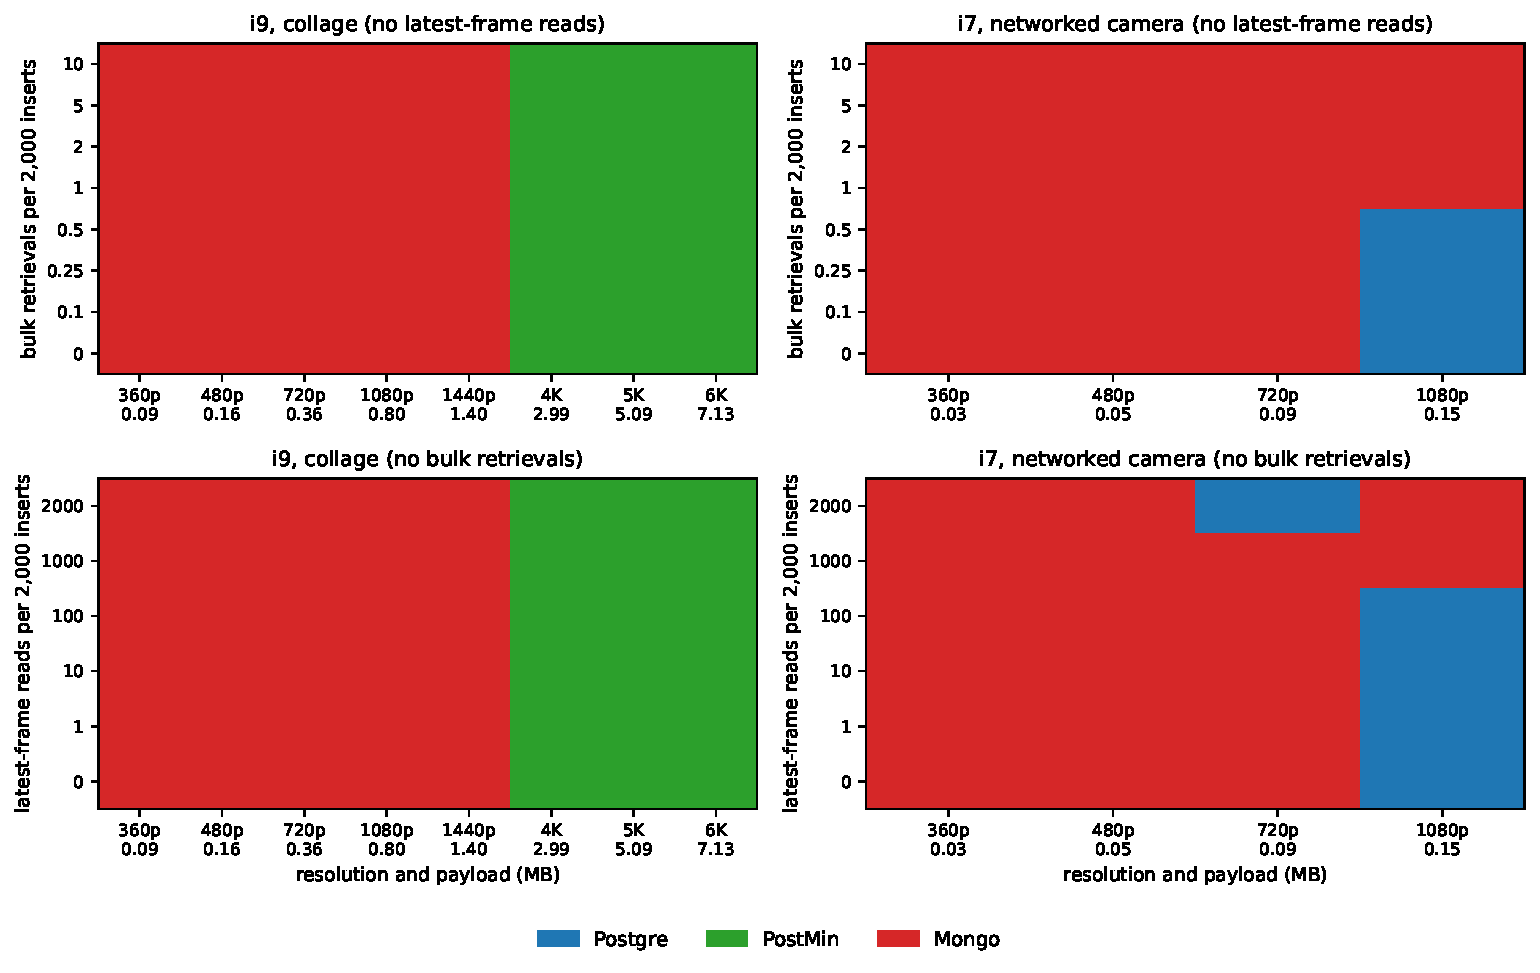
\includegraphics[width=\linewidth]{sensitivity_operation_mix.pdf}
\caption{Greenest architecture over payload (horizontal) and read frequency (vertical), for the collage on the larger host (left) and the networked camera's frames on the smaller host (right). Upper panels vary bulk retrievals with no latest-frame reads; lower panels vary latest-frame reads with no bulk retrievals.}\label{fig:mix}
\end{figure}

\section{Run-to-run variability}\label{sec:variability}
Each carbon value is a single integrated measurement over five runs, so it carries no dispersion of its own; the spread of the five timed runs bounds it (main text, Section~\ref{M-subsec:carbon_method}). We therefore perturbed every operation's carbon by a normal deviate whose coefficient of variation is that of its own timing (duration for insertion, latency for the reads), independently for each architecture and operation, and recorded how often the nominal winner stayed greenest over 20{,}000 draws. A winner that survives at least 95\% of draws is called robust. We use the full per-run spread rather than the standard error of the five-run mean, because the runs are not independent draws: on the smaller host they often slow down from one run to the next, and MongoDB's insertion at 720p on the collage took 2.9, 7.9, 8.5, 9.2 and 14.9~s. Table~\ref{tab:cv} gives the largest spread in each data set.

\begin{table}[htbp]
\centering
\caption{Largest run-to-run coefficient of variation in each data set, with the cell where it occurs.}\label{tab:cv}
\footnotesize\setlength{\tabcolsep}{4pt}
\begin{tabular}{@{}lll@{}}
\toprule
Data set & Insertion & Bulk retrieval \\
\midrule
\tabinput{../../sensitivity/tab_cv.tex}
\bottomrule
\end{tabular}
\end{table}

Every winner on the larger host is robust. The nine cells that are not (Table~\ref{tab:variability}) are all on the smaller host and all at a crossover, and in each the rival is the architecture that wins on the other side of it. Variability therefore blurs where a boundary falls; it does not change which architectures the boundary separates.

\begin{table}[htbp]
\centering
\caption{Winners that do not survive the perturbation: share of draws in which each architecture is greenest.}\label{tab:variability}
\footnotesize\setlength{\tabcolsep}{4pt}
\begin{tabular}{@{}lllll@{}}
\toprule
Data set & Payload & Mix & Greenest (share) & Closest rival (share) \\
\midrule
\tabinput{../../sensitivity/tab_variability.tex}
\bottomrule
\end{tabular}
\end{table}

\section{Embodied carbon of the retained frames}\label{sec:embodied}
The operational figures leave out the storage device (Table~\ref{M-tab:boundary} of the main text), yet a camera that keeps its frames needs capacity to hold them. For one camera at 5 frames per second, the retained volume is the payload times the measured storage amplification times the frames kept, for retention periods of 30, 90 and 365 days. Its embodied carbon uses the two per-gigabyte factors reported by \citet{tannu}: 0.16~kg~CO$_2$eq per GB for solid-state drives (the mean of 94 life-cycle reports, and the value used in the main text) and 0.02 for hard disks (the mean of 24); they are the only per-gigabyte factors in the sources the paper cites. The capacity is provisioned once and used for its whole life, so its embodied carbon is charged as a time share over a five-year drive life, the approach of the Software Carbon Intensity specification \citep{sci} and the five-year horizon Tannu and Nair use, and added to the operational carbon of a camera-year.

The measured amplification is used in two ways. MongoDB's reading falls far below 1 at small payloads, to 0.000 on distinct real frames at 360p and 480p. Each value is a single \texttt{collStats} reading taken straight after insertion, without forcing a checkpoint, so these measurements cannot settle whether it reflects compression or data not yet written to disk. The analysis is therefore run with amplification as measured and again with every value floored at 1.0. Footprints within 0.5\% of each other are treated as a tie.

Two results follow (Table~\ref{tab:embodied}). First, retained storage dwarfs the energy of writing it. Even 30 days of frames carry 4 to 16 times the operational carbon of the operational winner on hard disks, and 29 to 125 times on flash. For the deployment of the main text (1080p, 0.149~MB per frame, 90 days), that is about 23~kg a year per camera on hard disks and 185 to 191~kg on flash, against 1.7 to 3.6~kg of operational carbon. Second, this changes the choice only where the operational winner keeps more bytes than a close rival. At the deployment's own payload, inline PostgreSQL ($1.03\times$) wins ingestion but gives way to MongoDB after 2 to 8 days of retention on flash, or 18 to 65 days on hard disks, depending on the amplification basis. On the USB camera at 1080p, MongoDB ($1.03\times$) gives way to the hybrid ($1.00\times$) after 93 days on flash. On the smaller host's collage at 1440p, where the operational result is already a tie, MongoDB's measured $0.27\times$ would take the lead at once, but not on the floored basis. Everywhere else the operational winner also has the smallest footprint, or ties it, and the ranking stands. For any deployment that keeps frames for weeks, retention and storage amplification deserve as much attention as write energy.

\begin{table}[htbp]
\centering
\caption{Embodied carbon of the retained frames, ingestion-only profile. The third column is the embodied carbon of 30 days of frames divided by the operational carbon of the operational winner, over the payloads of each data set, on the floored basis. The last two columns list where, within a year of retention, the winner changes and to which architecture.}\label{tab:embodied}
\footnotesize
\begin{tabular}{@{}L{0.17\textwidth}lL{0.12\textwidth}L{0.24\textwidth}L{0.24\textwidth}@{}}
\toprule
Data set & Medium & Embodied ÷ operational at 30 days & Winner changes (amplification as measured) & Winner changes (amplification floored at 1.0) \\
\midrule
\tabinput{../../sensitivity/tab_embodied.tex}
\bottomrule
\end{tabular}
\end{table}

\section{Grid intensity and facility overhead}\label{sec:grid}
Emissions are energy multiplied by the grid's carbon intensity, so a change of grid scales every architecture by the same factor and cannot reorder them. Table~\ref{tab:grid} repeats the main text's cumulative comparison over 360p to 5K under seven national grids \citep{owid}: the hybrid has the lowest footprint under all of them, and only the absolute saving changes, from 0.07~g against MongoDB in Sweden to 1.16~g in India for this 2{,}000-frame-per-resolution workload. Power Usage Effectiveness multiplies every figure in the same way: at a PUE of 1.5 or 2.0 each value is 1.5 or 2 times the one shown, and the order is unchanged.

\begin{table}[htbp]
\centering
\caption{Cumulative footprint over 360p to 5K on the larger host (g CO$_2$eq), counting one insertion, one bulk retrieval and one latest-frame read at each resolution, at PUE 1.0. Bold marks the lowest in each row.}\label{tab:grid}
\small
\begin{tabular}{@{}lrrrr@{}}
\toprule
Grid & g/kWh & Postgre & PostMin & Mongo \\
\midrule
\tabinput{../../sensitivity/tab_grid.tex}
\bottomrule
\end{tabular}
\end{table}

\section{Frame rate, camera count and materiality}\label{sec:scale}
Annual carbon is the per-frame figure times the frames stored, so frame rate and camera count scale every architecture linearly and cannot reorder them; they decide how much the choice is worth. Table~\ref{tab:materiality} gives the annual ingestion carbon of one camera at 5 frames per second for two payloads, the deployment's measured 0.149~MB and the 4K collage, under three grids, with the saving against the runner-up and against the costliest architecture. For the deployment on the Indonesian grid, inline PostgreSQL saves 0.51~kg a year per camera against MongoDB (23\%) and 1.86~kg against the hybrid (52\%). At 4K the hybrid saves 26~kg against inline PostgreSQL (42\%) and 43~kg against MongoDB (54\%). Multiplying by 1.5 gives the figures at a PUE of 1.5.

\begin{table}[htbp]
\centering
\caption{Annual ingestion carbon of the greenest architecture for one camera at 5 frames per second (kg CO$_2$eq), and the saving against the runner-up and the costliest architecture, at PUE 1.0. The last column gives both savings for 100 cameras.}\label{tab:materiality}
\footnotesize
\setlength{\tabcolsep}{3pt}
\begin{tabular}{@{}lllllr@{}}
\toprule
Payload & Grid & Greenest (kg/yr) & Saving vs runner-up & Saving vs costliest & 100 cameras \\
\midrule
\tabinput{../../sensitivity/tab_materiality.tex}
\bottomrule
\end{tabular}
\end{table}

\section{Host, corpus and the worst case}\label{sec:host}
Table~\ref{tab:mix} already shows the winners in each of the six data sets. At small payloads the ordering is the same on both hosts and on every corpus; what moves is the payload at which the crossover falls (main text, Sections~\ref{M-subsec:twohosts} and~\ref{M-subsec:sizevsres}). Table~\ref{tab:worst} gives, for each architecture, its largest ratio to the greenest architecture at the same payload under the equal-weight profile. Inline PostgreSQL stays within 3.6 to 4.8 times the greenest on both hosts and every single camera, and within 1.4 times on the interleaved run; the hybrid reaches 12 to 39 times on the same five data sets, the price of its per-object HTTP request at small payloads. MongoDB's worst case is smaller still, but it is computed only over the payloads it could store: it fails at 6K on the larger host and from 4K on the smaller. Of the two architectures that complete every payload on both hosts, inline PostgreSQL therefore has the smaller worst case, which is the basis of its safe-default role in Table~\ref{M-tab:decision} of the main text.

\begin{table}[htbp]
\centering
\caption{Largest ratio of each architecture's equal-weight carbon to the greenest at the same payload, with the payload where it occurs.}\label{tab:worst}
\small
\begin{tabular}{@{}llll@{}}
\toprule
Data set & Postgre & PostMin & Mongo \\
\midrule
\tabinput{../../sensitivity/tab_worst.tex}
\bottomrule
\end{tabular}
\end{table}

\begin{thebibliography}{3}
\providecommand{\natexlab}[1]{#1}
\bibitem[Green Software Foundation(2024)]{sci}
Green Software Foundation (2024) Software Carbon Intensity (SCI) Specification. Published as ISO/IEC 21031:2024
\bibitem[Our World in Data(2024)]{owid}
Our World in Data (2024) Carbon intensity of electricity generation
\bibitem[Tannu and Nair(2023)]{tannu}
Tannu S, Nair PJ (2023) The dirty secret of SSDs: Embodied carbon. ACM SIGENERGY Energy Informatics Review 3(3):4--9. \url{https://doi.org/10.1145/3630614.3630616}
\end{thebibliography}

\end{document}
